\documentclass[border=10pt,tikz]{standalone}
\usepackage{amsmath}
\usepackage{amssymb}
\usepackage{bm}
\usepackage{tikz}
\usetikzlibrary{arrows.meta,calc,decorations.pathreplacing,patterns,shapes.geometric,positioning,shadings}

\definecolor{vacbg}{HTML}{0F1620}
\definecolor{platec}{HTML}{B8BCC2}
\definecolor{platedk}{HTML}{6B6E73}
\definecolor{standwave}{HTML}{EE6633}
\definecolor{contwave}{HTML}{F4C542}
\definecolor{forcec}{HTML}{FFEB99}

\begin{document}
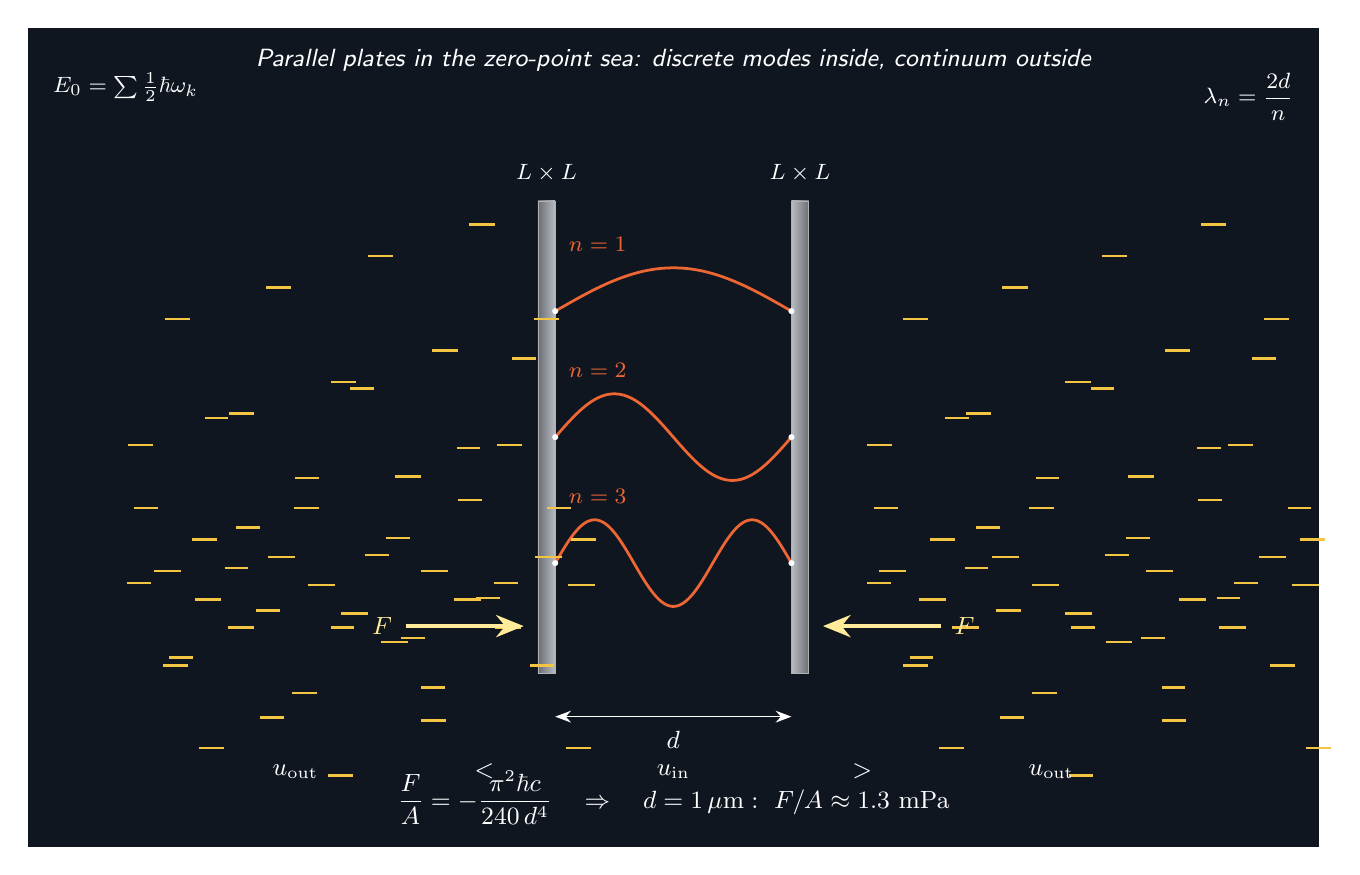
\begin{tikzpicture}[
  font=\sffamily,
  >={Stealth[length=3mm,width=2.4mm]}
]

% Dark vacuum background
\fill[vacbg] (-8.2,-5.2) rectangle (8.2,5.2);

% Title at top
\node[anchor=north, text=white, font=\sffamily\small\itshape] at (0,5.05)
  {Parallel plates in the zero-point sea: discrete modes inside, continuum outside};

% Geometry: plates centered at x = -1.5 and x = +1.5, so d = 3 units represents d
% plate thickness = 0.22, plate height = 6 (from y=-3 to y=3)

% Left plate (metallic gradient)
\shade[left color=platedk, right color=platec]
  (-1.72,-3) rectangle (-1.50,3);
\draw[line width=0.25pt, white!70!black] (-1.72,-3) rectangle (-1.50,3);

% Right plate
\shade[left color=platec, right color=platedk]
  (1.50,-3) rectangle (1.72,3);
\draw[line width=0.25pt, white!70!black] (1.50,-3) rectangle (1.72,3);

% Plate labels  L x L
\node[text=white, font=\sffamily\footnotesize] at (-1.61,3.35) {$L\times L$};
\node[text=white, font=\sffamily\footnotesize] at ( 1.61,3.35) {$L\times L$};

% Distance indicator d between plates (below plates)
\draw[white, line width=0.5pt, {Stealth[length=2mm]}-{Stealth[length=2mm]}]
  (-1.50,-3.55) -- (1.50,-3.55);
\node[text=white, font=\sffamily\small] at (0,-3.85) {$d$};

% ---- Standing waves between plates (red solid) ----
% Interior region: x from -1.50 to 1.50, length = 3 (this represents d).
% n=1 half-wavelength fits in d, so lambda_1 = 2d ; we plot sin(n*pi*(x+1.5)/3)
% Draw at 3 different y offsets so they don't overlap.

% n = 1, centered at y = 1.6
\draw[standwave, line width=1pt, smooth, samples=80, domain=-1.5:1.5]
  plot (\x, {1.6 + 0.55*sin(1*180*(\x+1.5)/3)});
\node[text=standwave, font=\sffamily\footnotesize, anchor=west] at (-1.45,2.45) {$n=1$};

% n = 2, centered at y = 0
\draw[standwave, line width=1pt, smooth, samples=120, domain=-1.5:1.5]
  plot (\x, {0.0 + 0.55*sin(2*180*(\x+1.5)/3)});
\node[text=standwave, font=\sffamily\footnotesize, anchor=west] at (-1.45,0.85) {$n=2$};

% n = 3, centered at y = -1.6
\draw[standwave, line width=1pt, smooth, samples=160, domain=-1.5:1.5]
  plot (\x, {-1.6 + 0.55*sin(3*180*(\x+1.5)/3)});
\node[text=standwave, font=\sffamily\footnotesize, anchor=west] at (-1.45,-0.75) {$n=3$};

% Nodes marked at x = -1.5 and x = 1.5 (small white dots)
\foreach \y in {-1.6,0,1.6} {
  \fill[white] (-1.50,\y) circle (1.1pt);
  \fill[white] ( 1.50,\y) circle (1.1pt);
}

% ---- Continuous spectrum outside (yellow short dense lines) ----
% Left side: x from -7.6 to -2.0 ; draw many short vertical/horizontal tiny lines
% Use randomish distribution via foreach to simulate continuum.
\foreach \i in {1,...,14} {
  \pgfmathsetmacro{\lx}{-7.4 + 0.43*\i + 0.04*mod(\i,3)}
  \pgfmathsetmacro{\ly}{ 2.7 - 0.40*mod(7*\i,11)}
  \draw[contwave, line width=0.9pt] (\lx,\ly) -- ({\lx+0.32},\ly);
}
\foreach \i in {1,...,14} {
  \pgfmathsetmacro{\lx}{-7.3 + 0.40*\i + 0.05*mod(\i,4)}
  \pgfmathsetmacro{\ly}{ 1.0 - 0.38*mod(5*\i,13)}
  \draw[contwave, line width=0.9pt] (\lx,\ly) -- ({\lx+0.30},\ly);
}
\foreach \i in {1,...,14} {
  \pgfmathsetmacro{\lx}{-7.4 + 0.42*\i + 0.04*mod(\i,5)}
  \pgfmathsetmacro{\ly}{-0.8 - 0.35*mod(3*\i,11)}
  \draw[contwave, line width=0.9pt] (\lx,\ly) -- ({\lx+0.31},\ly);
}
% extra sparser row near bottom
\foreach \i in {1,...,12} {
  \pgfmathsetmacro{\lx}{-7.1 + 0.48*\i + 0.03*mod(\i,3)}
  \pgfmathsetmacro{\ly}{-2.6 + 0.18*mod(5*\i,7)}
  \draw[contwave, line width=0.9pt] (\lx,\ly) -- ({\lx+0.34},\ly);
}

% Right side (mirror of above distribution)
\foreach \i in {1,...,14} {
  \pgfmathsetmacro{\lx}{2.0 + 0.42*\i + 0.04*mod(\i,3)}
  \pgfmathsetmacro{\ly}{ 2.7 - 0.40*mod(7*\i,11)}
  \draw[contwave, line width=0.9pt] (\lx,\ly) -- ({\lx+0.32},\ly);
}
\foreach \i in {1,...,14} {
  \pgfmathsetmacro{\lx}{2.1 + 0.40*\i + 0.05*mod(\i,4)}
  \pgfmathsetmacro{\ly}{ 1.0 - 0.38*mod(5*\i,13)}
  \draw[contwave, line width=0.9pt] (\lx,\ly) -- ({\lx+0.30},\ly);
}
\foreach \i in {1,...,14} {
  \pgfmathsetmacro{\lx}{2.0 + 0.42*\i + 0.04*mod(\i,5)}
  \pgfmathsetmacro{\ly}{-0.8 - 0.35*mod(3*\i,11)}
  \draw[contwave, line width=0.9pt] (\lx,\ly) -- ({\lx+0.31},\ly);
}
\foreach \i in {1,...,12} {
  \pgfmathsetmacro{\lx}{2.1 + 0.48*\i + 0.03*mod(\i,3)}
  \pgfmathsetmacro{\ly}{-2.6 + 0.18*mod(5*\i,7)}
  \draw[contwave, line width=0.9pt] (\lx,\ly) -- ({\lx+0.34},\ly);
}

% ---- Force arrows pointing inward toward center ----
\draw[forcec, line width=1.6pt, -{Stealth[length=3.5mm,width=2.8mm]}]
  (-3.4,-2.4) -- (-1.90,-2.4);
\node[text=forcec, font=\sffamily\small] at (-3.7,-2.4) {$F$};

\draw[forcec, line width=1.6pt, -{Stealth[length=3.5mm,width=2.8mm]}]
  (3.4,-2.4) -- (1.90,-2.4);
\node[text=forcec, font=\sffamily\small] at (3.7,-2.4) {$F$};

% ---- Energy density labels ----
\node[text=white, font=\sffamily\small] at (0,-4.25) {$u_{\mathrm{in}}$};
\node[text=white, font=\sffamily\small] at (-4.8,-4.25) {$u_{\mathrm{out}}$};
\node[text=white, font=\sffamily\small] at ( 4.8,-4.25) {$u_{\mathrm{out}}$};
\node[text=white, font=\sffamily\small] at (-2.4,-4.25) {$<$};
\node[text=white, font=\sffamily\small] at ( 2.4,-4.25) {$>$};

% Top-left info: zero-point sum
\node[text=white, anchor=north west, font=\sffamily\footnotesize]
  at (-8.0,4.75) {$E_0=\sum\tfrac12\hbar\omega_k$};

% Top-right info: standing-wave condition
\node[text=white, anchor=north east, font=\sffamily\footnotesize]
  at (8.0,4.75) {$\lambda_n=\dfrac{2d}{n}$};

% Bottom formula: Casimir pressure
\node[text=white, anchor=south, font=\sffamily\small]
  at (0,-5.05) {$\dfrac{F}{A}=-\dfrac{\pi^{2}\hbar c}{240\,d^{4}}\quad\Rightarrow\quad d=1\,\mu\mathrm{m}:\ F/A\approx 1.3\ \mathrm{mPa}$};

\end{tikzpicture}
\end{document}
